
\clearpage  
\onecolumn  

\section{Missing proofs for prediction error metric} 

\begin{lemma} [Lemma \ref{lem:necessity-of-error-properties}]
A deterministic $c$-approximate ($c > 0$) algorithm exists for problem (\ref{problem}), only if (1) the prediction error is finite, i.e., $\tilde{d}_B(A) = 0 \iff {d}_B(A), \forall A, B \subseteq N$ and (2) the error is directional consistent, i.e., $\tilde{d}_B(A) \cdot {d}_B(A) \geq 0, \forall A, B \subseteq N$.
\end{lemma} 
\begin{proof}
We first show that the error must be finite. Construct two simple instances of problem (\ref{problem}) $I_1$ and $I_2$ as follows. Both instances have $N = \{ a, b \}$ and $K = 1$. Instance $I_1$ has $f(\{a\}) = 1, f(\{b\}) = 0$; instance $I_2$ has $f(\{ a \}) = 0$, $f(\{ b \}) = 1$. The optimal value for both instances is $1$. Suppose the algorithm can access a predictor $\tilde{f}$ with $\tilde{f}(\emptyset) = 0, \tilde{f}(\{a\}) = 1, \tilde{f}(\{b\}) = 1$. Any deterministic algorithm returns either set $\{ a \}$ or $\{ b \}$ or $\emptyset$, producing a value of $0$ for $I_2$ if returning set $\{ a \}$ or $0$ for $I_1$ if returning set $\{ b \}$ or $0$ for both. This is, at best, a $0$-approximate algorithm. The argument also holds with $\tilde{f}(\emptyset) = \tilde{f}(\{a\}) = \tilde{f}(\{b\}) = 0$. Therefore, we must have $\tilde{d}_B(A) = 0 \iff {d}_B(A), \forall A, B \subseteq N$ to construct a $c$-approximate ($c > 0$) algorithm. 

We then show that the error must be directional and consistent using a similar construction. This time, instance $I_1$ has $f(\{a\}) = 1, f(\{b\}) = -1$; instance $I_2$ has $f(\{ a \}) = -1$, $f(\{ b \}) = 1$. The optimal value for both instances is still $1$. Suppose that $\tilde{f}(\emptyset) = 0, \tilde{f}(\{a\}) = 1, \tilde{f}(\{b\}) = 1$. Any deterministic algorithm returns either set $\{ a \}$ or $\{ b \}$ or $\emptyset$, producing a value of $-1$ for $I_2$ if returning set $\{ a \}$ or $-1$ for $I_1$ if returning set $\{ b \}$ or $0$ for both. Again, this is, at best, a $0$-approximate algorithm. 
\end{proof}

\begin{lemma} [Lemma \ref{lem:any-epsilon-error-can-be-infite-eta}]
For any fixed $0 < \epsilon < 1$, there exists a $\epsilon$-erroneous predictor $\tilde{f}$ with an infinite $\eta$. 
\end{lemma}
\begin{proof}
Let $N = \{a, b\}, f(\emptyset) = 0, f(\{a\}) = 1, f(\{ b \}) = \frac{2\epsilon}{1 - \epsilon}, f(\{ a, b \}) = \frac{1 + \epsilon}{1 - \epsilon}, \tilde{f}(\emptyset) = 0, \tilde{f}(\{ a \}) = 1 + \epsilon, \tilde{f}(\{ b \}) = \frac{2 \epsilon}{1 - \epsilon}, \tilde{f}(\{ a, b \}) = 1 + \epsilon$. This yields a $\epsilon$-erroneous predictor $\tilde{f}$ with an infinite $\eta$, as $d_{\{ b \}}(\{ a \}) = \frac{2 \epsilon}{1 - \epsilon}$ and $\tilde{d}_{\{ b \}}(\{ a \}) = 0$. 
\end{proof}

\begin{lemma} [Lemma \ref{lem:any-eta-error-has-bounded-epsilon-error}]
Any predictor $\tilde{f}$ for a non-negative function $f$ with a total prediction error $\eta = \eta_u \cdot \eta_o$ is $\epsilon$-erroneous with $\epsilon \leq \max \{ 1 - \frac{1}{\eta_u}, \eta_o - 1 \}$. 
\end{lemma}
\begin{proof}
For any $S \subseteq N$, we have $\frac{d_{\emptyset}(S)}{\eta_u} \leq \tilde{d}_{\emptyset}(S) \leq \eta_o \cdot d_{\emptyset}(S) \Rightarrow \frac{f(S)}{\eta_u} \leq \tilde{f}(S) \leq \eta_o \cdot f(S) \Rightarrow \frac{1}{\eta_u} - 1 \leq \frac{\tilde{f}(S) - f(S)}{f(S)} \leq \eta_o - 1 \Rightarrow \frac{|\tilde{f}(S) - f(S)|}{f(S)} \leq \max \{ 1 - \frac{1}{\eta_u}, \eta_o - 1 \}$.  
\end{proof}


\section{Analysis for the single-step predictive greedy heuristic}

\begin{algorithm}
\caption{Single-step Predictive Greedy} \label{single-step-greedy-algo}
\begin{algorithmic}[1]
\State \textbf{Input:} finite set $N$, marginal gain predictions $\tilde{d}$, and the cardinality constraint $K$
\State \textbf{Output:} set $S$ with $|S| \leq K$
\State initialize $S^0 \gets \emptyset$, $t \gets 0$

\While{$|S^{t}| < K$}
    \State let $e_t \in N - S^t$ such that $\tilde{d}_{\{e_t\}}(S^{t}) = \max_{e \in {N - S^t}}{\tilde{d}_{\{e\}}(S^{t})}$, with ties break arbitrarily
    \State $\tilde{d}_{t} \gets \tilde{d}_{\{e_t\}}(S^{t})$, ${d}_{t} \gets {d}_{\{e_t\}}(S^{t})$
    \If{$\tilde{d}_{t} > 0$}
        \State $S^{t+1} \gets S^{t} \cup \{ e_t \}$, $t \gets t + 1$ \Comment{add $e_t$ to set $S^{t}$}
    \Else 
        \State \textbf{break} \Comment{stop with set $S^{t}$}
    \EndIf 
\EndWhile
\State $K^* \gets |S^{t}|$ \Comment{$K^*$ is the size of the output set with $K^* \leq K$}
\State \textbf{return} \( S^{t} \)
\end{algorithmic}
\end{algorithm}

Let $F^{\textsf{OPT}}$ be the value of an optimal solution to problem (\ref{problem}) and $F^{\textsf{PG}}$ the value of a particular solution constructed by Algorithm \ref{single-step-greedy-algo}. We assume $K^* \geq 1$ to exclude trivial problems with $F^{\textsf{PG}} = F^{\textsf{OPT}} = 0$, where $\tilde{d}_{0} \leq 0$ indicates $d_{\{e\}}(\emptyset) \leq 0, \forall e \in N$ and $F^{\textsf{OPT}} = f(\emptyset) = 0$ due to the directional consistency of the errors. We begin with the following property for general submodular set functions: 

\begin{lemma} [\cite{greedySubmodularFunctions}] \label{lem:bound-property}
If $f$ is a submodular set function on $N$ with $\theta(f) = - \min_{S \subseteq N, e \in N - S}{d_{\{e\}}{(S)}}$, then
\[ f(T) \leq f(S) + \sum_{e \in T - S}{d_{\{e\}}(S)} + |S-T| \theta(f), ~~~ \forall S, T \subseteq N \]
\end{lemma}

%We introduce the $\theta$ function, where $-\theta(f)$ denotes the minimum value of any single element's marginal gain, i.e.,  
%$\theta(f) = - \min_{S \subseteq N, e \in N - S}{d_{\{e\}}{(S)}}$.
%The function $f$ is non-decreasing if and only if $\theta(f) \leq 0$. The bound on $F^{\textsf{PG}}$ is a function in the value $\theta(f)$. 


\begin{lemma} \label{lem:bounds on f(S^t)}
\[ F^{\textsf{OPT}} \leq f(S^t) + K \cdot \eta \cdot d_{t} + t \cdot \max \{ 0, \theta(f) \}, ~~~ t = 0, ..., K^*-1 ~(\textit{including } K^* \textit{ if } K^* < K) \]
\end{lemma}
\begin{proof}
Fix any $t = 0, ..., K^* - 1 ~(\textit{including } K^* \textit{ if } K^* < K)$. 
For any $e \in N - S^t$, we have $\tilde{d}_{\{e\}}(S^{t}) \leq \tilde{d}_{\{e_t\}}(S^{t})$, by the selection of $e_t$. Therefore, it holds that:
\[ d_{\{e\}}(S^t) \leq \eta_u \cdot \tilde{d}_{\{e\}}(S^{t}) \leq \eta_u \cdot \tilde{d}_{\{e_t\}}(S^{t}) \leq \eta_u \cdot \eta_o \cdot {d}_{\{e_t\}}(S^{t}) = \eta \cdot d_t \]
Let $T$ be the optimal set to problem (\ref{problem}). We have $\tilde{d}_t > 0 \Rightarrow d_t > 0$ and $\sum_{e \in T - S^t}{d_{\{e\}}(S^t)} \leq \sum_{e \in T - S^t}{\eta \cdot d_t} \leq |T - S^t| \cdot \eta \cdot d_t \leq K \cdot \eta \cdot d_t$.
We have $|S^t-T| \theta(f) \leq |S^t-T| \cdot \max \{ 0, \theta(f) \} \leq t \cdot \max \{ 0, \theta(f) \}$. 
By Lemma \ref{lem:bound-property}, we have:
\[ F^{\textsf{OPT}} \leq f(S^t) + \sum_{e \in T - S^t}{d_{\{e\}}(S^t)} + |S^t-T| \theta(f) \leq f(S^t) + K \cdot \eta \cdot d_{t} + t \cdot \max \{ 0, \theta(f) \} \qedhere \]
\end{proof}


\begin{theorem} [Bounds on Single-step Predictive Greedy] \label{thm:bounds-on-SPG}
If the single-step predictive greedy is applied and stops after $K^* \leq K$ steps, we have:
\begin{align*}
& \frac{F^{\textsf{PG}} + K^* \cdot \max \{ 0, \theta(f) \}}{F^{\textsf{OPT}}} \geq 1,           & K^* < K\\
& \frac{F^{\textsf{PG}} + K \cdot \max \{ 0, \theta(f) \}}{F^{\textsf{OPT}}} \geq 1 - (1 - \frac{1}{\eta K})^K,  & K^* = K
\end{align*}
\end{theorem}
\begin{proof}
\textbf{Case 1 ($K^* < K$).} Let $T$ be the optimal set to problem (\ref{problem}). We have $\tilde{d}_{K^*} \leq 0 \Rightarrow {d}_{K^*} \leq 0$. By Lemma \ref{lem:bounds on f(S^t)}, $F^{\textsf{OPT}} \leq f(S^{K^*}) + K \cdot \eta \cdot d_{K^*} + K^* \cdot \max \{ 0, \theta(f) \} \leq F^{\textsf{PG}} + K^* \cdot \max \{ 0, \theta(f) \}$.

\textbf{Case 2 ($K^* = K$).} Let $\alpha = 1 - \frac{1}{\eta K}$. By Lemma \ref{lem:bounds on f(S^t)}, we have:
\[ F^{\textsf{OPT}} \leq f(S^t) + K \cdot \eta \cdot d_{t} + t \cdot \max \{ 0, \theta(f) \}, ~~~ t = 0, ..., K-1 \]
Substituting $\alpha = 1 - \frac{1}{\eta K}$ and $d_t = f(S^{t+1}) - f(S^t)$, multiplying by $\alpha^{K-t-1}$ for the $t$-th inequality, and re-arranging gives:
\[ \alpha^{K-t-1} f(S^{t+1}) \geq \alpha^{K-t} \cdot f(S^t) - {\max \{ 0, \theta(f) \}} \cdot (1 - \alpha) \cdot \alpha^{K-t-1} \cdot t + {F^{\textsf{OPT}}} \cdot (1 - \alpha) \cdot \alpha^{K-t-1} \]
for $t = 0, ..., K-1$. Summing all the inequalities (with $f(S^0) = f(\emptyset) = 0$), we have:
\begin{align*}
    F^{\textsf{PG}} = f(S^K) &\geq - {\max \{ 0, \theta(f) \}} \cdot (1 - \alpha) \cdot \sum_{t=0}^{K-1}{\alpha^{K-t-1} \cdot t} + {F^{\textsf{OPT}}} \cdot (1 - \alpha) \cdot \sum_{t=0}^{K-1}{\alpha^{K-t-1}} \\
    &= - {\max \{ 0, \theta(f) \}} \cdot (-\sum_{t=0}^{K-1}{\alpha^t} + K) + F^{\textsf{OPT}} \cdot (1 - \alpha^K) \\
    &\geq - {\max \{ 0, \theta(f) \}} \cdot K + F^{\textsf{OPT}} \cdot (1 - \alpha^K) \qedhere
\end{align*}
\end{proof}

Theorem \ref{thm:bounds-on-SPG} implies that, for any non-decreasing $f$ (i.e., $\theta(f) \leq 0$), $F^{\textsf{PG}} = F^{\textsf{OPT}}$, meaning the single-step predictive greedy gives an optimal solution when the output has cardinality less than $K$. 
If the predictions are perfect, i.e., $\eta = 1$, the approximation ratio matches that of the single-step greedy heuristic with perfect information \cite{greedySubmodularFunctions}. Therefore, the single-step predictive greedy achieves optimal consistency. Observe that $1 - (1 - \frac{1}{\eta K})^K > 1 - \lim_{K \rightarrow \infty}{(1 - \frac{1}{\eta K})^K} \geq 1 - e^{-1/\eta}$. Therefore, Theorem \ref{thm:bounds-on-SPG} shows that, for any non-decreasing $f$ (i.e., $\theta(f) \leq 0$), we have:
\[ \frac{F^{\textsf{PG}}}{F^{\textsf{OPT}}} \geq 1 - (1 - \frac{1}{\eta K})^K > 1 - e^{-1/\eta} \]
The analysis hold if we re-define the prediction error to be the maximum multiplicative gap between any single-element's marginal gain and its prediction, i.e., Theorem \ref{thm:bounds-on-SPG} holds if we let $\eta_u = \max_{A \subseteq N, e \in N}{\frac{d_{\{e\}}(A)}{\tilde{d}_{\{e\}}(A)}}, \eta_o = \max_{A \subseteq N, e \in N}{\frac{\tilde{d}_{\{ e \}}(A)}{d_{\{e\}}(A)}}$, and $\eta = \eta_u \cdot \eta_o$.


\section{Missing proofs for optimization with predictions} \label{appendix:proof-section-3}

\begin{theorem} [Theorem \ref{thm:bounds-on-RPG-submodular-predictors}]
If the R-step predictive greedy is applied with a submodular predictor $\tilde{f}$ and returns a set of cardinality $K^* \leq K$, we have:
\begin{align*}
& \frac{F^{\textsf{RPG}} + K^* \cdot \max \{ 0, \frac{\theta(\tilde{f})}{\lambda_o} \}}{F^{\textsf{OPT}}} \geq \frac{1}{\lambda},           & K^* < K\\
& \frac{F^{\textsf{RPG}} + K \cdot \max \{ 0, \frac{\theta(\tilde{f})}{\lambda_o} \}}{F^{\textsf{OPT}}} \geq \frac{1}{\lambda} \cdot ( 1 - (1 - \frac{1}{{\lceil \frac{K}{R} \rceil}})^{\lceil \frac{K}{R} \rceil}),  & K^* = K
\end{align*}
\end{theorem}
\begin{proof}
Let $S$, $T$, and $\tilde{T}$ denote the set returned by the R-step greedy heuristic, the optimal set to problem (\ref{problem}) to maximize function $f$, and the optimal set to problem (\ref{problem}) to maximize function $\tilde{f}$. Let ${{\tilde{F}}^{\textsf{RPG}}} = \tilde{f}(S)$ and ${\tilde{F}^{\textsf{OPT}}} = \tilde{f}(\tilde{T})$. We have:
\[ F^{\textsf{RPG}} = f(S) \geq \lambda_o \cdot \tilde{f}(S) = \lambda_o \cdot {\tilde{F}}^{\textsf{RPG}} ~\text{and}~ F^{\textsf{OPT}} = f(T) \leq \frac{1}{\lambda_u} \cdot \tilde{f}(T) \leq \frac{1}{\lambda_u} \cdot \tilde{f}(\tilde{T}) = \frac{1}{\lambda_u} \cdot {\tilde{F}^{\textsf{OPT}}} \]
Since $\tilde{f}$ is accessible to the algorithm, applying Theorem \ref{thm:bounds-on-RPG} with $\eta = 1$ gives: 
\[ \frac{F^{\textsf{RPG}} + K^* \max \{ 0, \frac{\theta(\tilde{f})}{\lambda_o} \}}{F^{\textsf{OPT}}} \geq \frac{\lambda_o {\tilde{F}}^{\textsf{RPG}} + K^* \max \{ 0, \frac{\theta(\tilde{f})}{\lambda_o} \}}{\frac{1}{\lambda_u} \cdot {\tilde{F}^{\textsf{OPT}}}} = \frac{1}{\lambda} \cdot \frac{{\tilde{F}}^{\textsf{RPG}} + K^* \max \{ 0, {\theta(\tilde{f})} \}}{{\tilde{F}^{\textsf{OPT}}}} \geq \frac{1}{\lambda} \]
if $K^* < K$. Similarly, we have, for $K^* = K$:
\[ \frac{F^{\textsf{RPG}} + K \cdot \max \{ 0, \frac{\theta(\tilde{f})}{\lambda_o} \}}{F^{\textsf{OPT}}} \geq \frac{\lambda_o {\tilde{F}}^{\textsf{RPG}} + K \cdot \max \{ 0, \frac{\theta(\tilde{f})}{\lambda_o} \}}{\frac{1}{\lambda_u} \cdot {\tilde{F}^{\textsf{OPT}}}} \geq \frac{1}{\lambda} \cdot ( 1 - (1 - \frac{1}{{\lceil \frac{K}{R} \rceil}})^{\lceil \frac{K}{R} \rceil}) \qedhere \]
\end{proof}

\newpage
\section{Supplementary material for experiment: ML feature selection} \label{appendix:supp-material-application1}

\subsection{Descriptions of data and benchmarks} \label{appendix:descriptions-data-benchmarks}

The "airline passenger satisfaction" dataset, available on Kaggle (\url{https://www.kaggle.com/datasets/teejmahal20/airline-passenger-satisfaction}), is the source of our primary dataset. Our dataset, motivated by the research conducted by Jiang et al. \cite{jiang2022forecast}, documents the experiences of 129,880 customers who took flights with American Airlines in 2015. The data have 23 attributes that span anything from complex flight details to simple passenger demographics. These characteristics are heterogeneous, spanning from qualitative sequential factors to numerical continuous variables, and they document different facets of the passengers' experiences \cite{jiang2022forecast}. By examining these specifics, we can identify important factors affecting passengers' satisfaction, dissatisfaction, or neutrality toward their travels. In addition, a well-annotated breast cancer dataset from Kaggle (\url{https://www.kaggle.com/datasets/yasserh/breast-cancer-dataset}) was used as the second dataset. Although this dataset was used for classification models in Assegie et al. \cite{assegie2021breast} and other predictive modeling studies, it has a distinct use in our work. We aim to use this dataset to test and evaluate a new feature selection process. For making comparable analysis, our experimental setup includes a range of baseline models and an independent erroneous oracle to evaluate feature selection methodologies in various scenarios thoroughly. The baselines were selected to encompass a range of typical feature selection strategies, creating a solid comparative framework to determine the effectiveness of the oracle method. 


\subsubsection*{Benchmarks description}

\textit{SelectKBest}: Select the top K features or variables from a given dataset and use a univariate feature selection technique that assesses the statistical significance between each feature and the target variable using the ANOVA F-value \cite{otchere2022application}. 

\textit{Recursive Feature Elimination (RFE)}: This uses a backward selection process to delete features based on their relevance \cite{sachdeva2022systematic}, which is evaluated using a tree classifier in our experiment. It was widely employed in classification and regression problems, as the selected features were updated iteratively to find features contribute significantly \cite{abdulkareem2021evaluation,chen2018decision}.

\textit{Mutual Information}: Quantifies the information shared between two random variables and the relationship between feature subset and the target variable, considering linear and nonlinear connections \cite{vergara2014review}.

\textit{Extra Trees}: Employs an ensemble of decision trees, namely the Extra Trees Classifier, to evaluate the significance of each feature. The calculation of feature importance is based on the reduction in impurity that each feature brings across all trees in the forest \cite{sharaff2019extra}. 


\subsection{Implementations for the single-step and the R-step predictive greedy} \label{appendix:experiment1-implementations}

\paragraph{Single-step predictive greedy.} 
The pseudo-code of single-step predictive greedy feature selection is given by Algorithm \ref{algo:oracle-simulation}. 

\begin{algorithm}[ht!]
\caption{Single-Step Predictive Greedy Feature Selection} \label{algo:oracle-simulation}
\begin{algorithmic}[1]
\State \textbf{Input:} Training data: \( X_{\text{train}}, y_{\text{train}} \), test data: \( X_{\text{test}}, y_{\text{test}} \), feature count \( K \), error bounds \( \eta_u, \eta_o \)
\State \textbf{Output:} Set \( S \) of selected features with performance metrics

\State Initialize \( S \gets \emptyset \), \( N \gets \) set of all features
\State Initialize an empty list \( \text{Accuracies} \)

\While{\( |S| < K \)}
    \State Calculate \( A_{\text{base}} \) from training on \( S \) (or set to 0 if \( S \) is empty)
    \State Initialize an empty list \( \text{Gains} \) to store feature gains and subsets' accuracies
    \For{each \( f \) in \( N \setminus S \)}
        \State Create new feature subset \( S' \gets S \cup \{f\} \)
        \State Train with \( S' \) to obtain \( A_{\text{ext}} \)
        \State Calculate the actual gain: \( \text{gain} \gets A_{\text{ext}} - A_{\text{base}} \)
        \State Apply prediction error: \( \text{gain}_{\text{pred}} \gets \text{gain} \cdot \text{generate\_error}(\eta_u, \eta_o) \)
        \State Append \( (f, S', A_{\text{ext}}, \text{gain}, \text{gain}_{\text{pred}}) \) to \( \text{Gains} \)
    \EndFor
    \State Sort \( \text{Gains} \) by \( \text{gain}_{\text{pred}} \) in descending order
    \State Select the feature with the highest predicted gain: \( f_{\text{sel}}, S_{\text{sel}} \gets \text{Gains}[0][0], \text{Gains}[0][1] \)
    \State Update \( S \gets S_{\text{sel}} \) and remove \( f_{\text{sel}} \) from \( N \)
    \State Train on \( S \) to update \( A_{\text{new}} \)
    \State Append \( A_{\text{new}} \) to \( \text{Accuracies} \)
\EndWhile
\State \Return \( \text{Accuracies} \)
\end{algorithmic}
\end{algorithm}


\paragraph{R-step predictive greedy.} The R-step predictive greedy method involves iteratively constructing feature subsets using a combination strategy that maximizes predictive gain. It is highly inefficient for choosing an extensive number of features, as it uses a layered combination and evaluation methodology. In our experiment, the feature number is insignificant. The R-step predictive greedy algorithm aligns with theoretical perspectives. The pseudo-code of the R-step predictive greedy feature selection is given by Algorithm \ref{algo:r-step-predictive-greedy}. 

\begin{algorithm}[ht!]
\caption{R-Step Predictive Greedy Feature Selection} \label{algo:r-step-predictive-greedy}
\begin{algorithmic}[1]
\State \textbf{Input:} Training data: \( X_{\text{train}}, y_{\text{train}} \), test data: \( X_{\text{test}}, y_{\text{test}} \), feature count \( K \), step size \( R \), error bounds \( \eta_u, \eta_o \)
\State \textbf{Output:} Set \( S \) of selected features with performance metrics

\State Initialize \( S \gets \emptyset \), \( N \gets \) set of all features
\State Initialize an empty list \( \text{A} \)

\While{\( |S| < K \)}
    \If{\( |S| + R > K \)}
        \State \( R \gets K - |S| \) \Comment{Adjust R if remaining features to select are less than R}
    \EndIf
    \State Initialize \( Gain_\text{best} \gets -\infty \), \( C_\text{best} \gets \text{null} \)
    \State \( A_\text{base} \gets \) train on \( S \) (or set to 0 if \( S \) is empty)
    
    \State Form all possible combinations of \( R \) features from \( N \setminus S \)
    \For{each combination \( C \) of \( R \) features}
        \State \( F_\text{ext} \gets S \cup C \)
        \State \( A_\text{ext} \gets \) train on \( F_\text{ext} \)
        \State \( \text{Gain} \gets (A_\text{ext} - A_\text{base}) \cdot \text{generate\_error}(\eta_u, \eta_o) \)
        
        \If{\( \text{Gain} > Gain_\text{best} \)}
            \State \( Gain_\text{best} \gets \text{Gain} \)
            \State \( C_\text{best} \gets C \)
        \EndIf
    \EndFor
    
    \State \( S \gets S \cup  C_\text{best} \)
    \State Remove \(  C_\text{best} \) from \( N \)
    \State \( A_\text{new} \gets \) train on \( S \)
    \State Append \( A_\text{new} \) to \( A \)
\EndWhile

\State \Return \( \text{Accuracies} \)
\end{algorithmic}
\end{algorithm}


\clearpage
\section{Supplementary material for experiment: Influence maximization} \label{appendix:supp-material-application2}

\subsection{Implementation details} \label{appendix:experiment2-implementation-details}
The experiment is conducted on real-world networks from Twitter\footnote{\url{https://snap.stanford.edu/data/ego-Twitter.html}}\cite{facebook&twitter} (nodes: 81,306, directed edges: 1,768,149), Reddit\footnote{\url{https://snap.stanford.edu/data/soc-RedditHyperlinks.html}}\cite{reddit} (nodes: 55,863, directed edges: 858,490), and Facebook\footnote{\url{https://snap.stanford.edu/data/ego-Facebook.html}}\footnote{\url{https://snap.stanford.edu/data/gemsec-Facebook.html}}\cite{facebook&twitter,facebook2} (nodes: 4,039, undirected edges: 88,234; nodes: 50,515, edges: 819,306).

For undirected graphs, we treated the edges as bidirectional. We used the edges provided by these datasets to create networks to be tested in our experiment. For the Greedy algorithm, we selected the Nodes in $K$ iterations, each time selecting the remaining node with the largest influence, defined as the number of the selected node and its adjacent nodes that are not yet active. This involves activating the selected nodes and their inactive adjacent nodes,  adding the number of new activated nodes, and removing the selected node from the candidate pool for the next iteration. SOP-Greedy follows the same selection process without knowing the true influence of each node when making the iteration. Given the prediction errors $\eta_n, \eta_o$ and the practical influence $\xi_n$, we set the predicted influence $\xi^*_n \gets \xi_n \cdot \exp(Y)$ with $Y \sim \mathcal{U}(-\log \eta_u, \log \eta_o)$. The node with the maximum predicted influence, $ \xi^* $, is chosen in each iteration. For RSOP-Greedy, instead of considering only one node choice at a time, we consider all combinations of up to $R$ nodes from the available candidates in each iteration. The practical influence of each combination of $R$ nodes is the number of these $R$ nodes and all their adjacent nodes that are not yet active. Similarly, we obtain the predicted influence of each combination using the same method as in SOP-Greedy. For Weighted Random, the weight is the out-degree of each node. The probability of selecting node $n$ is $p_n = \frac{d_n}{\sum_{j=1}^N d_j}$, where $d_n$ is the out-degree of node $n$. For Random, each node has an equal probability of being selected. After selecting the $K$ nodes by each method, we measure the number of affected nodes of all selected nodes and their adjacent nodes.


\subsection{Experiments on large-scale networks}


\label{appendix:large-scale}
\begin{figure}[htbp]
    \centering
    % First figure
    \begin{minipage}{0.245\textwidth}
        \centering
        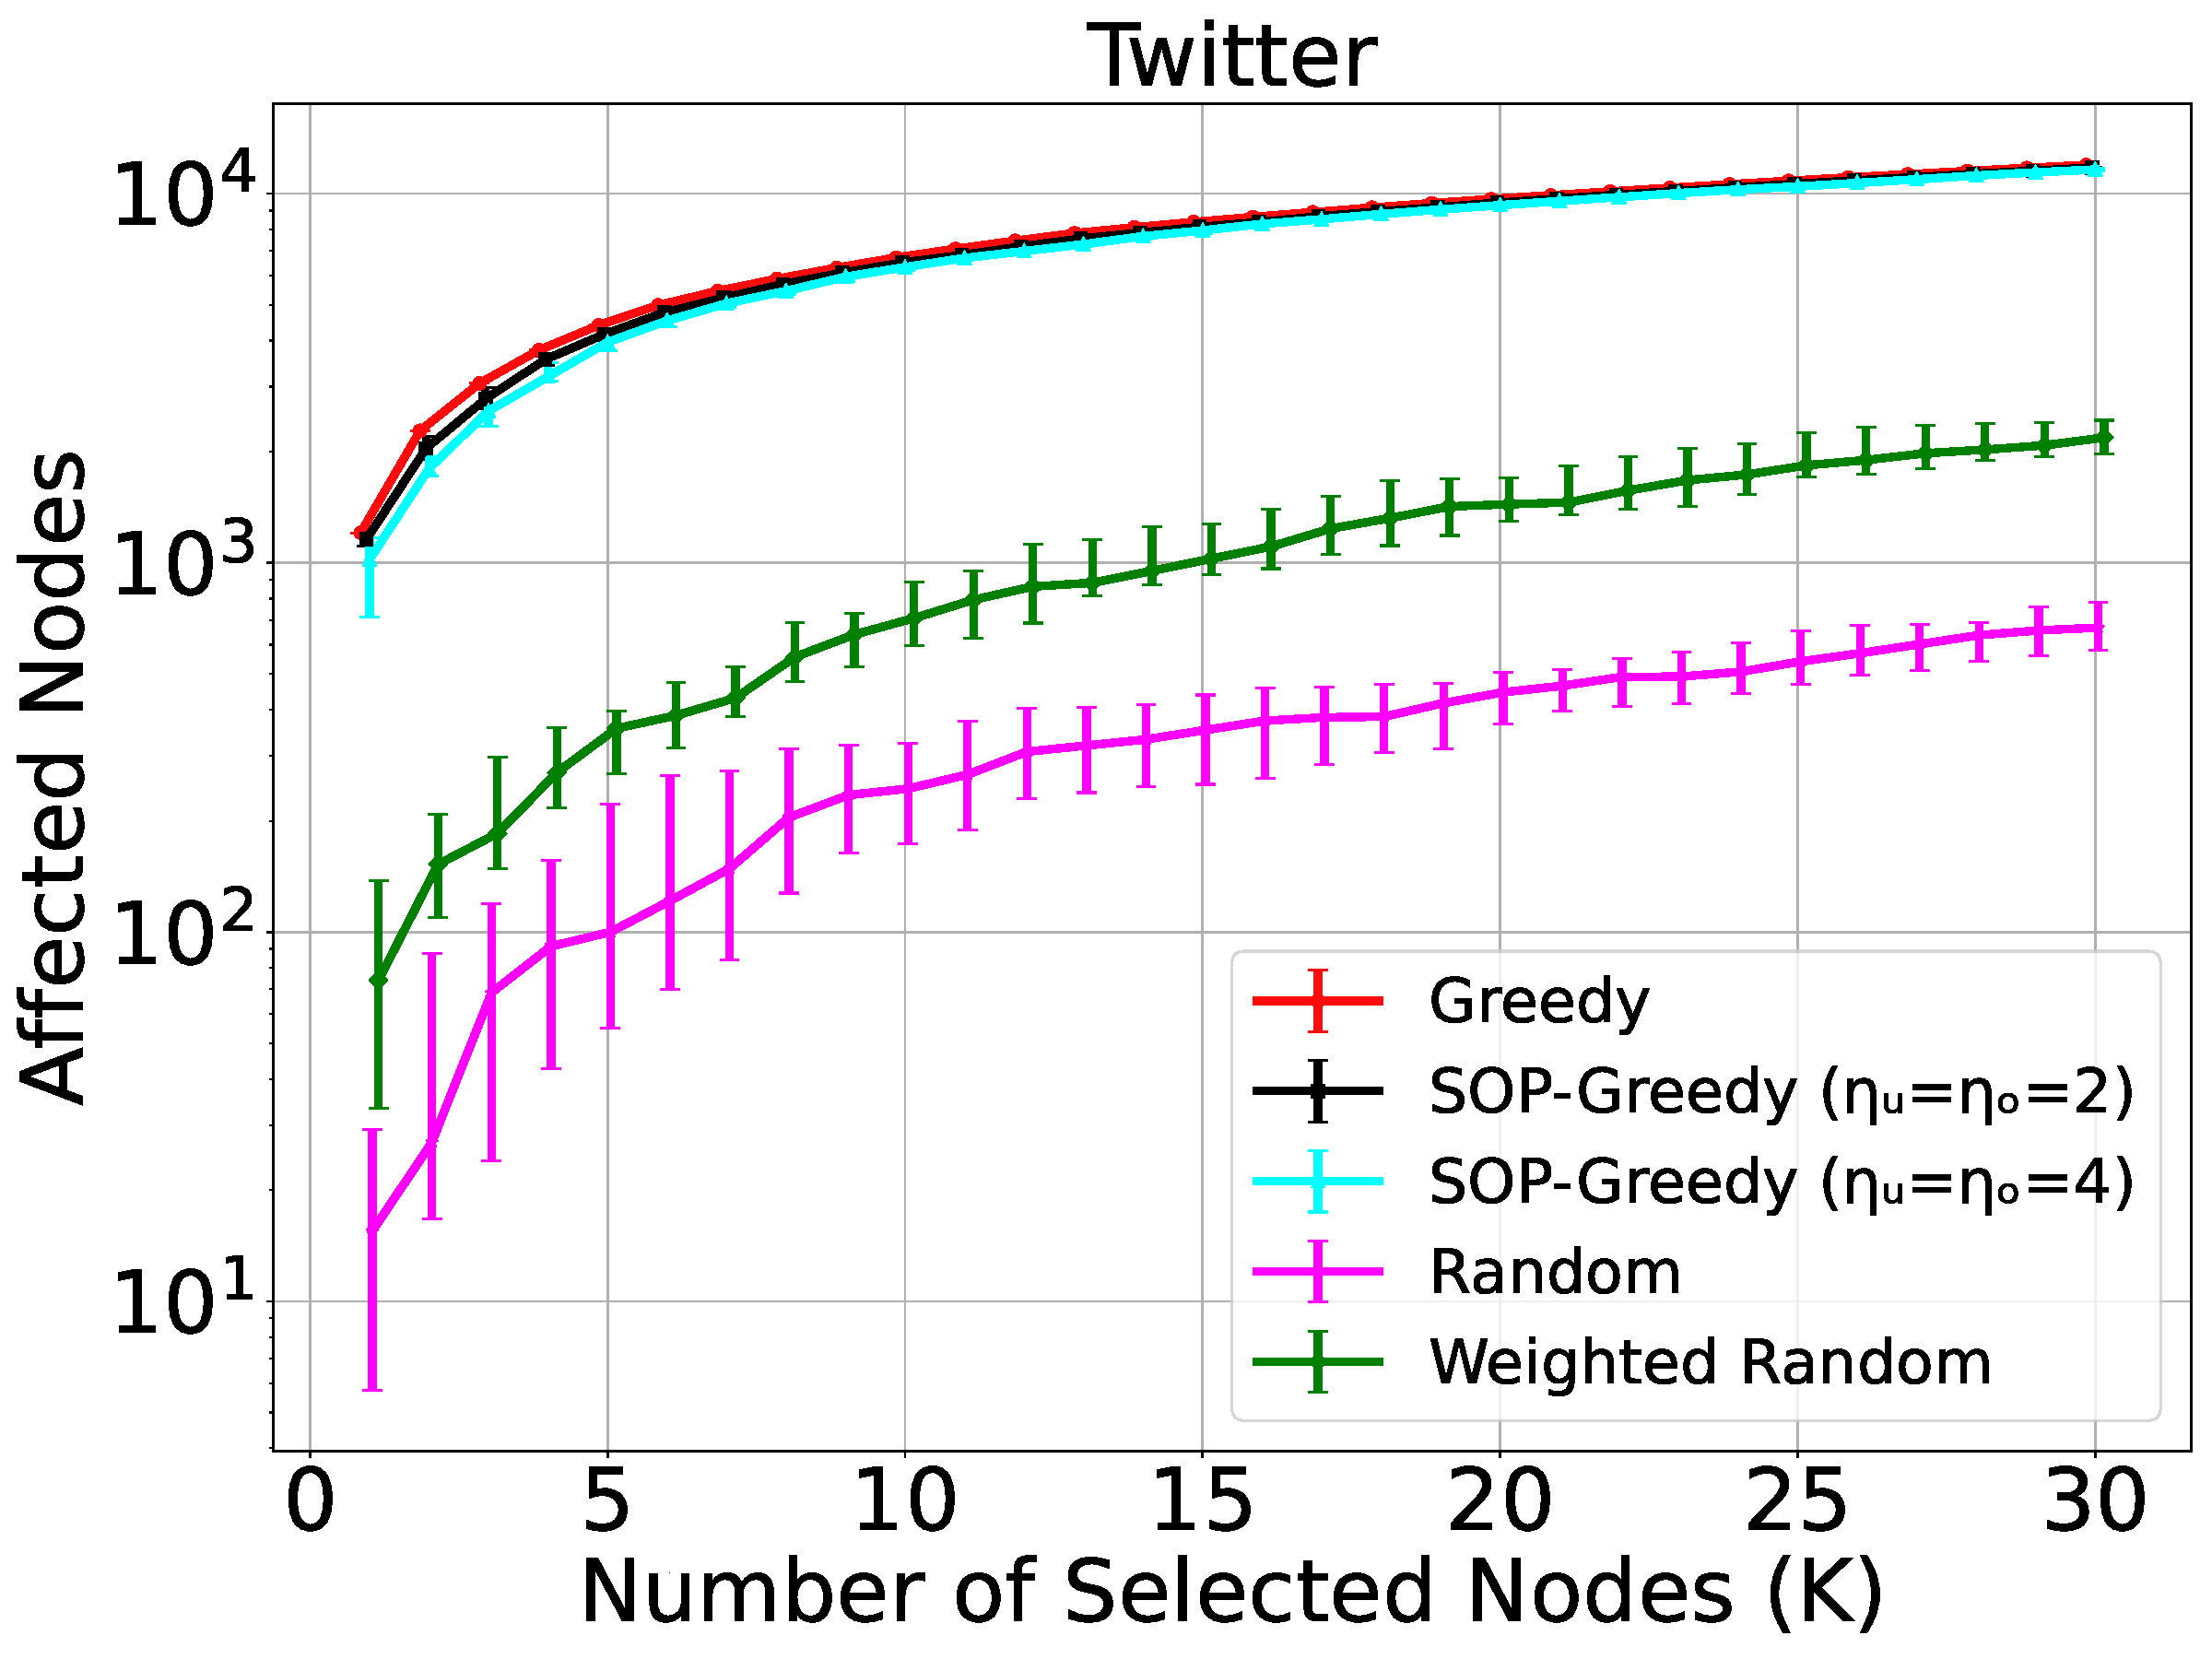
\includegraphics[width=\linewidth]{Figures/GraphExperiment/log_comparison/log_twt.pdf}
        \label{fig:log_twt}
    \end{minipage}\hfill
    % Second figure
    \begin{minipage}{0.245\textwidth}
        \centering
        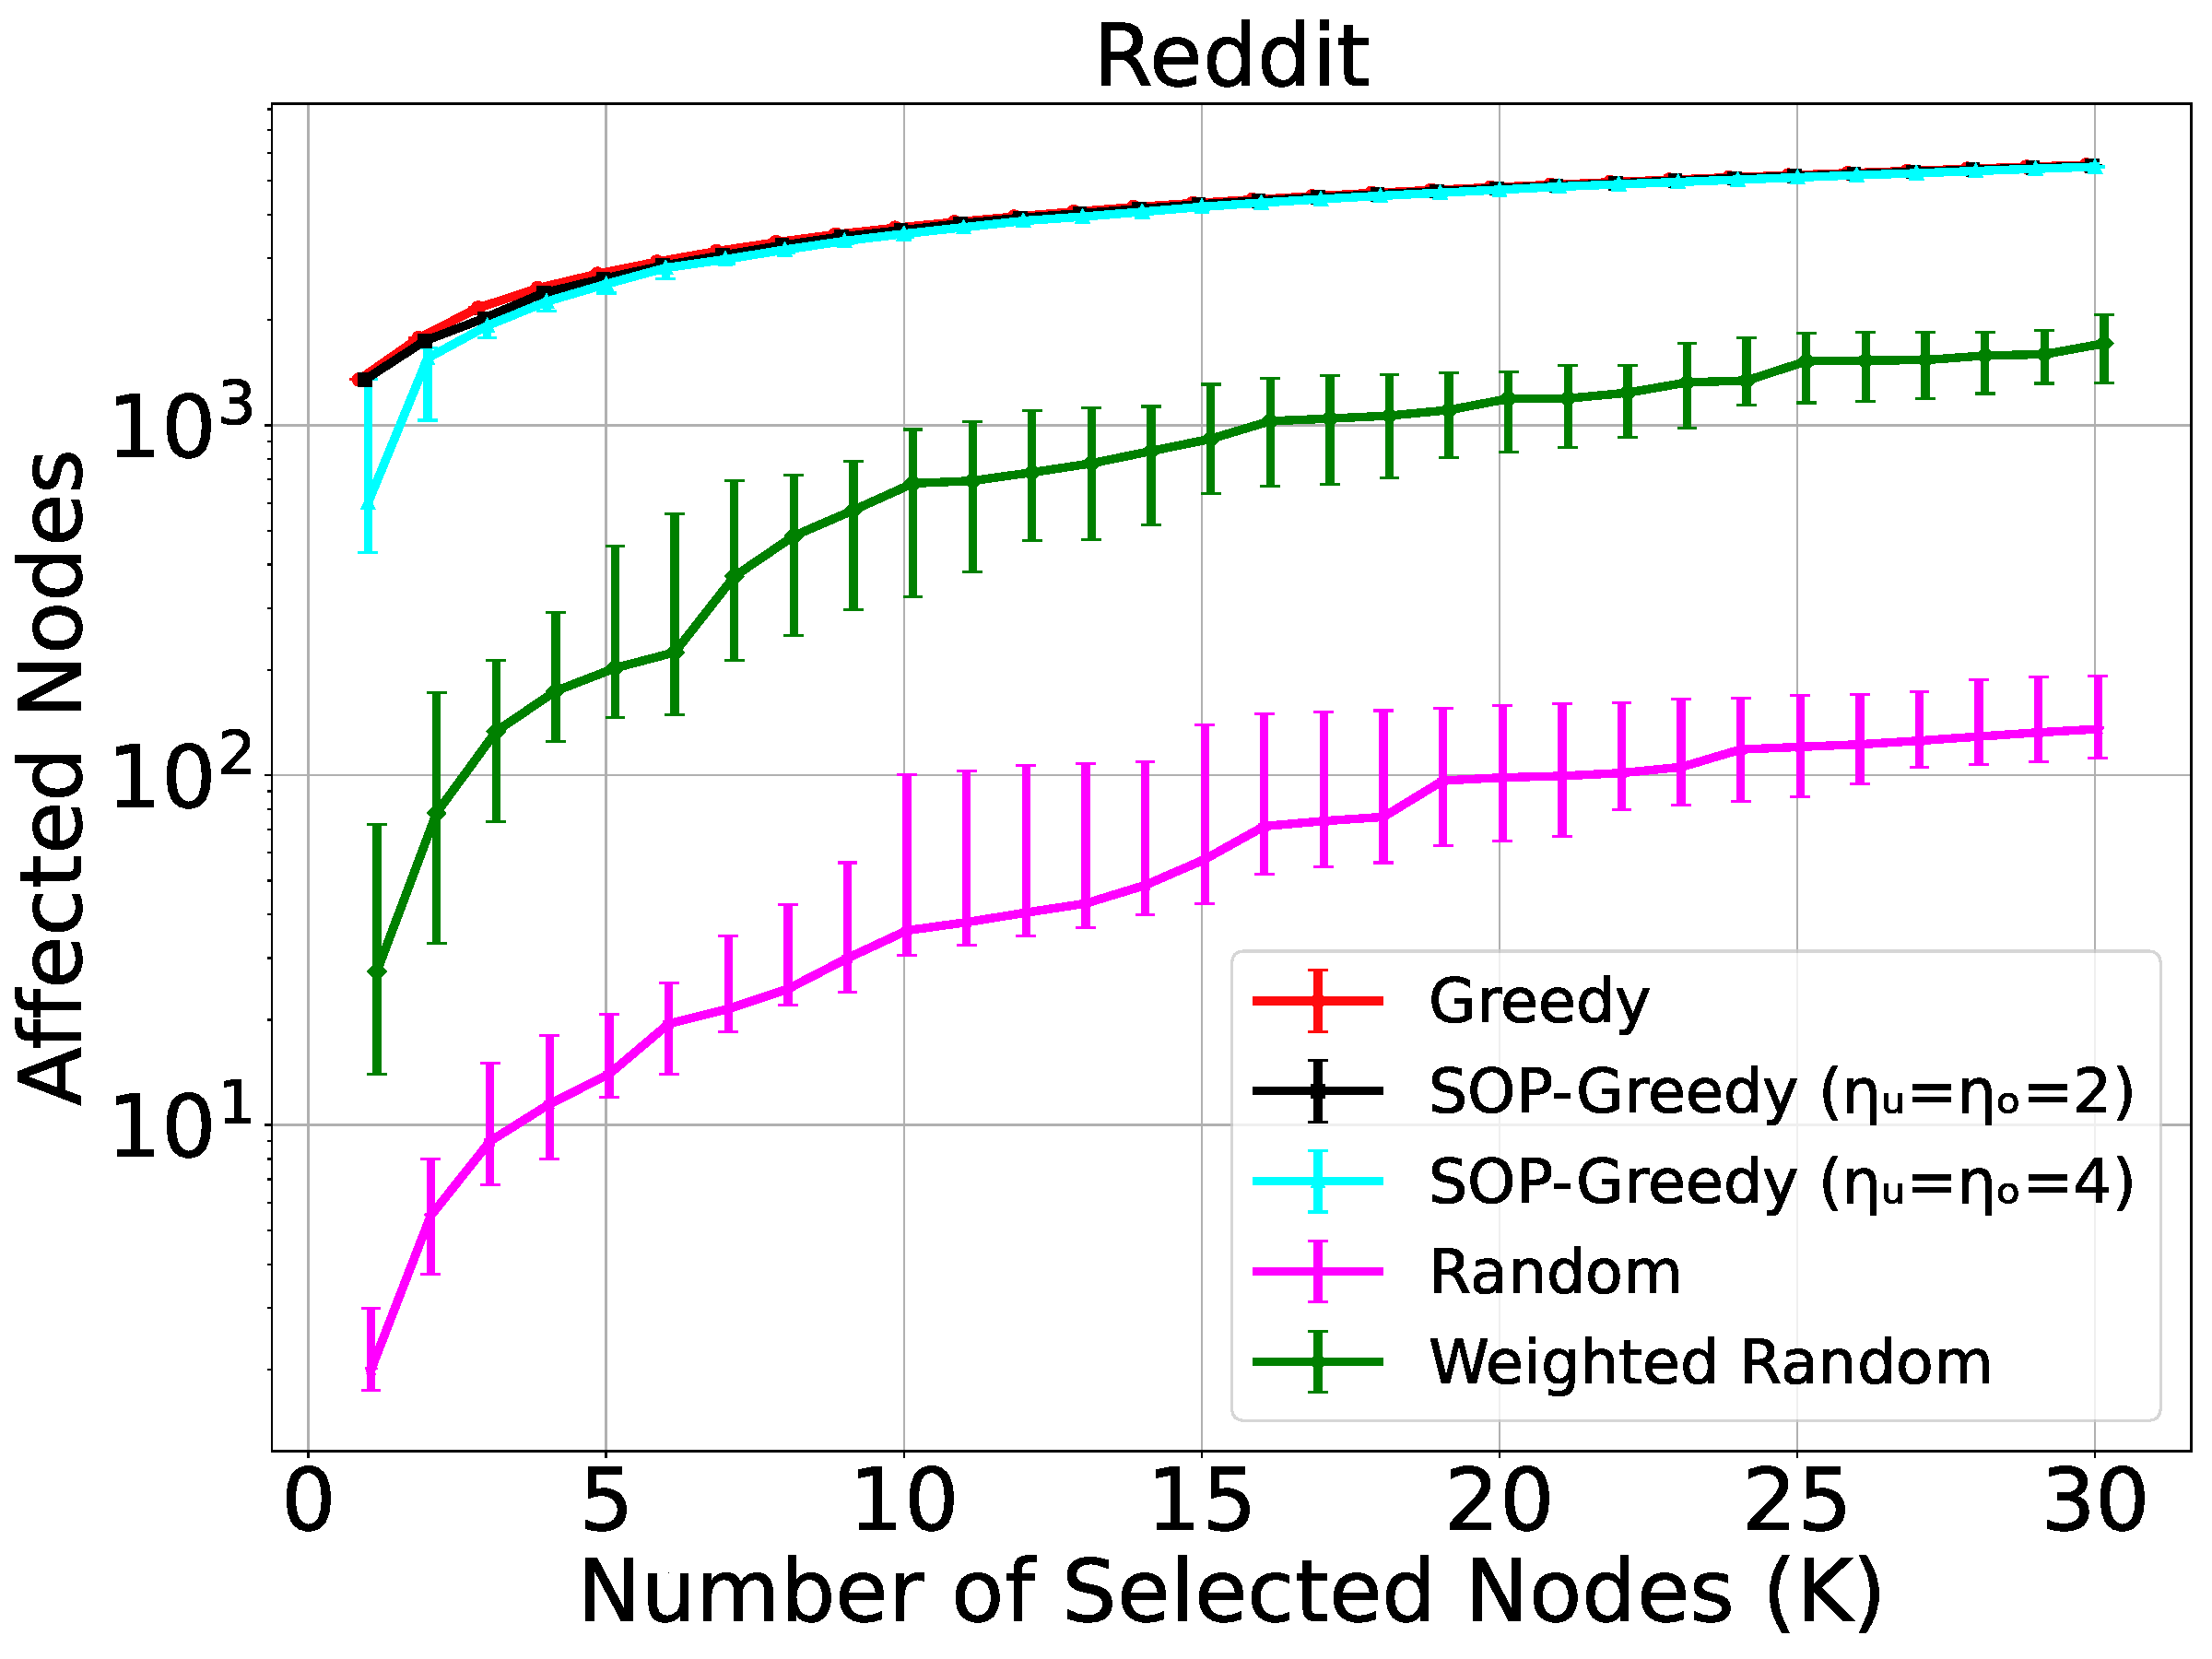
\includegraphics[width=\linewidth]{Figures/GraphExperiment/log_comparison/log_rdt.pdf}
        \label{fig:log_rdt}
    \end{minipage}
    \hfill
    % Third figure
    \begin{minipage}{0.245\textwidth}
        \centering
        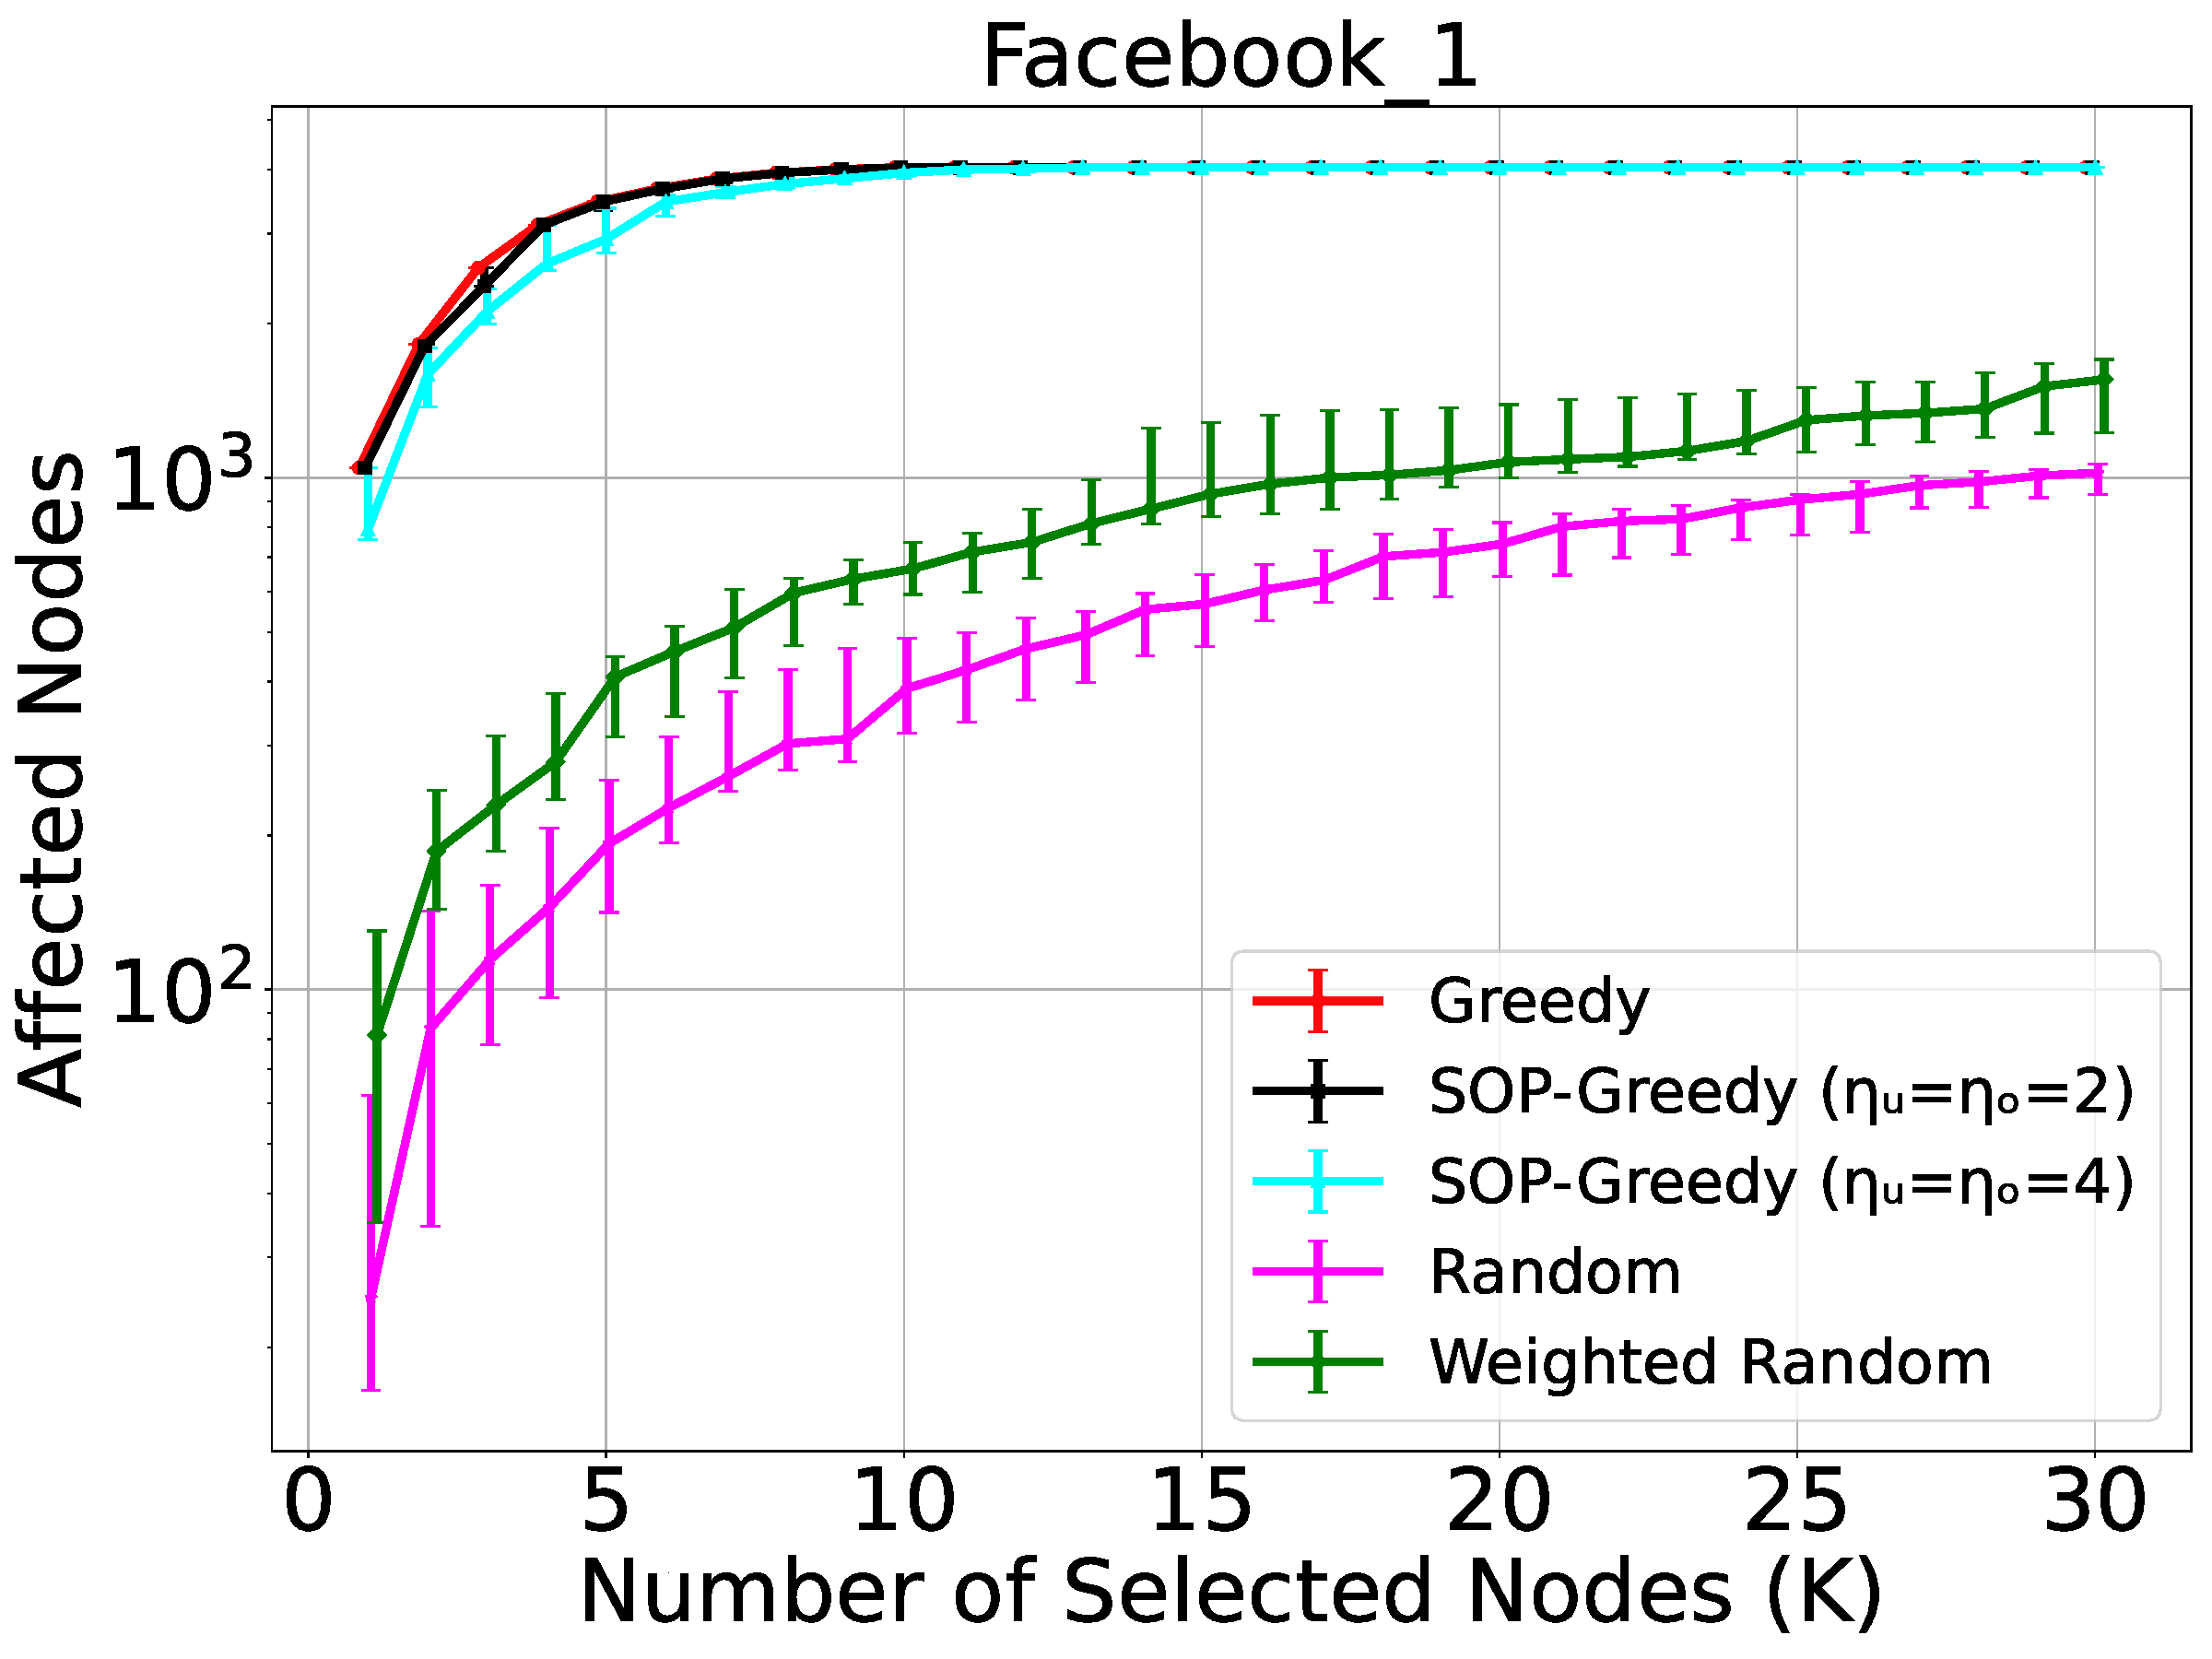
\includegraphics[width=\linewidth]{Figures/GraphExperiment/log_comparison/log_fb1.pdf}
        \label{fig:log_fb1}
    \end{minipage}
    \hfill
    % Fourth figure
    \begin{minipage}{0.245\textwidth}
        \centering
        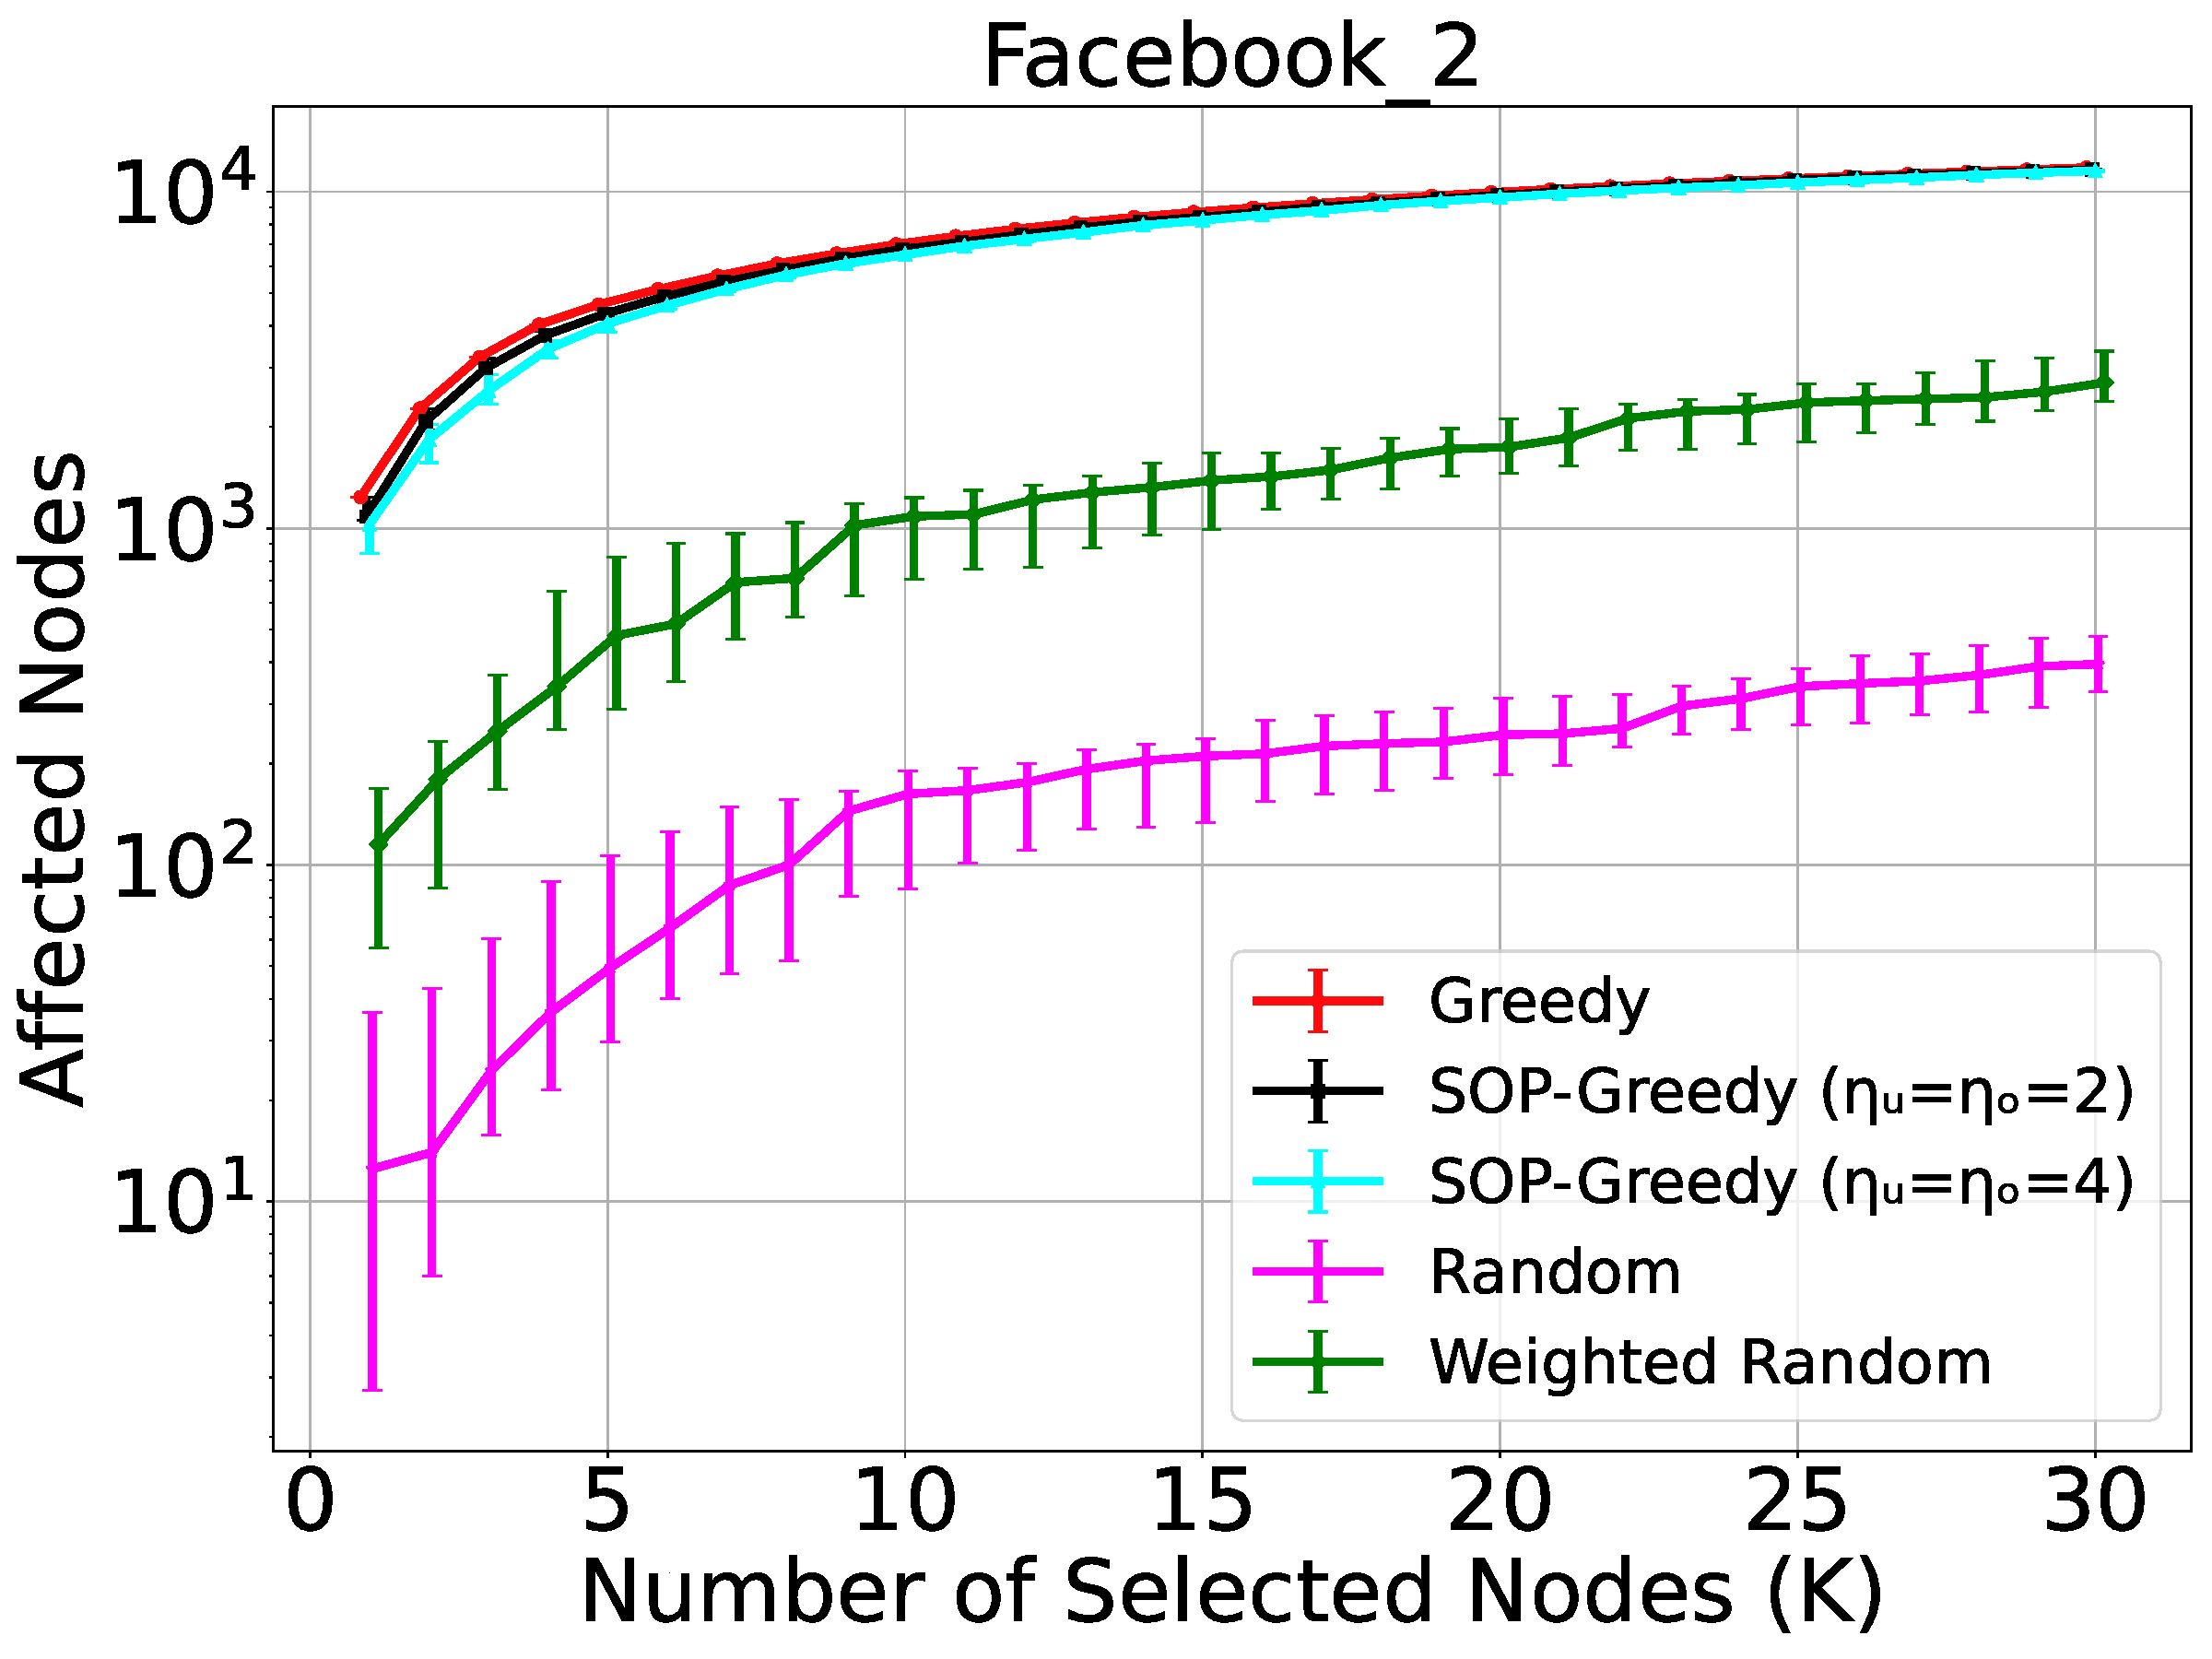
\includegraphics[width=\linewidth]{Figures/GraphExperiment/log_comparison/log_fb2.pdf}
        \label{fig:log_fb2}
    \end{minipage}
    \caption{Affected nodes with an increasing $K$ on large-scale networks.}
    \label{fig:large-scale}
\end{figure}


Figure \ref{fig:large-scale} presents the affected nodes for different algorithms on four networks with varying $K$. This experiment uses large-scale real-world network data. RSOP-Greedy is excluded here due to its complexity. Instead, two groups of SOP-Greedy with different prediction accuracies are provided. According to the observations, the performance difference between RSOP-Greedy and SOP-Greedy is minimal. The higher prediction error only makes a difference when $K$ is small; as $K$ increases, they tend to demonstrate similar performance. Greedy consistently achieves the strongest performance due to complete information, but the advantage of Greedy vanishes quickly as $K$ increases. All greedy-based algorithms show significant advantages over Weighted Random and Random. The overall result matches our previous experiments on small-scale real-world networks (Figure \ref{fig:2stp}).







\newpage
\section{Supplementary material for experiment: Text summarization} \label{appendix:supp-material-application3}


\subsection{Implementation details} \label{appendix:experiment3-implementation-details}

\textbf{Converge alpha value.}
In text summarization, the parameter $\alpha$ is vital for regulating the saturation degree of information coverage in the coverage function. It finds a balance between covering new material and avoiding repetition. We use a methodical technique that includes testing out several values of $\alpha$, from 0.5 to 10, to determine the best $\alpha$. To carry out this experiment, we compare the results of each $\alpha$ to reference summaries and use the ROUGE-1 F-Measure to determine how well the summaries are. We have found that it is sensible to choose an $\alpha$ equals to 1 as the BBC news sports might have more concentrated thematic content or repetitive information. It suggests that when $\alpha>1$, the converge function still capture the essential content effectively. The results is inconsistent with the previous research work \cite{lin2011class} since the dataset's characteristics are different. 


\textbf{Diversity clusters.}
While Lin et al.,(2020) \cite{lin2011class} uses varied clustering depending on the document's complexity and length, our experiment uses a basic clustering approach to text summarizing since the majority of the articles in our dataset are short and only contain a few phrases. Applying Lin's proposed huge number of clusters \cite{lin2011class}, which are meant for more complicated or lengthy papers, may not be possible or successful given the short character of these texts. Alternatively, we opt to employ a predetermined, modest cluster size (e.g., 2-3). Without making the process of summary too complicated, this approach seeks to capture the most salient thematic distinctions within the texts. 



\textbf{Prediction error application.}
For coverage objective function, the prediction error is applied element-wise to each similarity score between items between pairs $(i, j)$ (where $i \in V$ and $j \in S$). By simulating the effect of each element's contribution under uncertainty, this method approximates the effect of individual elements' prediction uncertainty on the total coverage metric. For diversity objective function, the prediction error is applied to each similarity interaction within the clusters, which simulates the effect of uncertainty within coherent subgroups of the dataset. For facility location objective function, the prediction error is applied to the maximum similarity score for each item in $V$ relative to the set $S$, incorporating prediction error into the most influential comparison evaluations. 
Consequently, each objective function's practical needs and theoretical foundations should be considered when deciding how to use prediction error.






\textbf{Submodular optimization.}
The third experiment was performed by Algorithm \ref{algo:greedy_text_sum}.


\begin{algorithm}
\caption{Greedy Submodular Maximization for Text Summarization} 
\label{algo:greedy_text_sum}
\begin{algorithmic}[1]
\State \textbf{Input:} $V, k, \text{func}, \alpha, \eta_u, \eta_o$
\State \textbf{Output:} a set of selected sentences $S$

\Procedure{GreedyMaximization}{$V, k, \text{func}, \alpha, \eta_u, \eta_o$}
    \State $S \gets \emptyset$
    \While{$|S| < k$}
        \State $s \gets \arg\max_{x \in V \setminus S} \text{CalculateSubmodularValue}(S \cup \{x\}, V, \text{func}, \alpha, \eta_u, \eta_o)$
        \State $S \gets S \cup \{s\}$
    \EndWhile
    \State \textbf{return} $S$
\EndProcedure

\Function{CalculateSubmodularValue}{$S, V, \text{func}, \alpha, \eta_u, \eta_o$}
    \State $value \gets 0$
    \If{$\text{func} = \text{``coverage''}$}
        \For{$i \in V$}
            \State $sum\_within\_S \gets 0$
            \For{$j \in S$}
            \State $error \gets 1$
            \If{$\eta_u \neq \text{None}$ and $\eta_o \neq \text{None}$}
                \State $error \gets \text{generate\_error}(\eta_u, \eta_o)$
            \EndIf
            \State $sum\_within\_S \gets sum\_within\_S + w_{ij} \cdot error$
        \EndFor
        \State $sum\_overall \gets \sum_{k \in V} w_{ik}$
        \State $covered\_value \gets \min(sum\_within\_S, \alpha \cdot sum\_overall)$
        \State $value \gets value + covered\_value$
    \EndFor
    \ElsIf{$\text{func} = \text{``diversity''}$}
        \For{$cluster \in \text{clusters}$}
            \State $cluster\_intersection \gets cluster \cap S$
            \If{$cluster\_intersection$}
                \State $cluster\_similarity \gets 0$
                \For{$i \in cluster, j \in cluster\_intersection$}
                    \State $error \gets 1$
                    \If{$\eta_u \neq \text{None}$ and $\eta_o \neq \text{None}$}
                        \State $error \gets \text{generate\_error}(\eta_u, \eta_o)$
                    \EndIf
                    \State $sim \gets w_{ij} \cdot error$
                    \State $cluster\_similarity \gets cluster\_similarity + sim$
                \EndFor
                \State $diversity\_score \gets diversity\_score + \sqrt{\frac{cluster\_similarity}{|V|}}$
            \EndIf
        \EndFor
        \State $value \gets -diversity\_score$
    \ElsIf{$\text{func} = \text{``facility\_location''}$}
        \For{$i \in V$}
            \State $max\_val \gets \max_{j \in S} w_{ij}$
            \State $error \gets 1$
            \If{$\eta_u \neq \text{None}$ and $\eta_o \neq \text{None}$}
                \State $error \gets \text{generate\_error}(\eta_u, \eta_o)$
            \EndIf
            \State $value \gets value + max\_val \cdot error$
        \EndFor
    \EndIf
    \State \textbf{return} $value$
\EndFunction

\end{algorithmic}
\end{algorithm}


\newpage
\subsection{Results} \label{appendix:experiment3-more-results}


\begin{figure} [ht!]
    \centering
    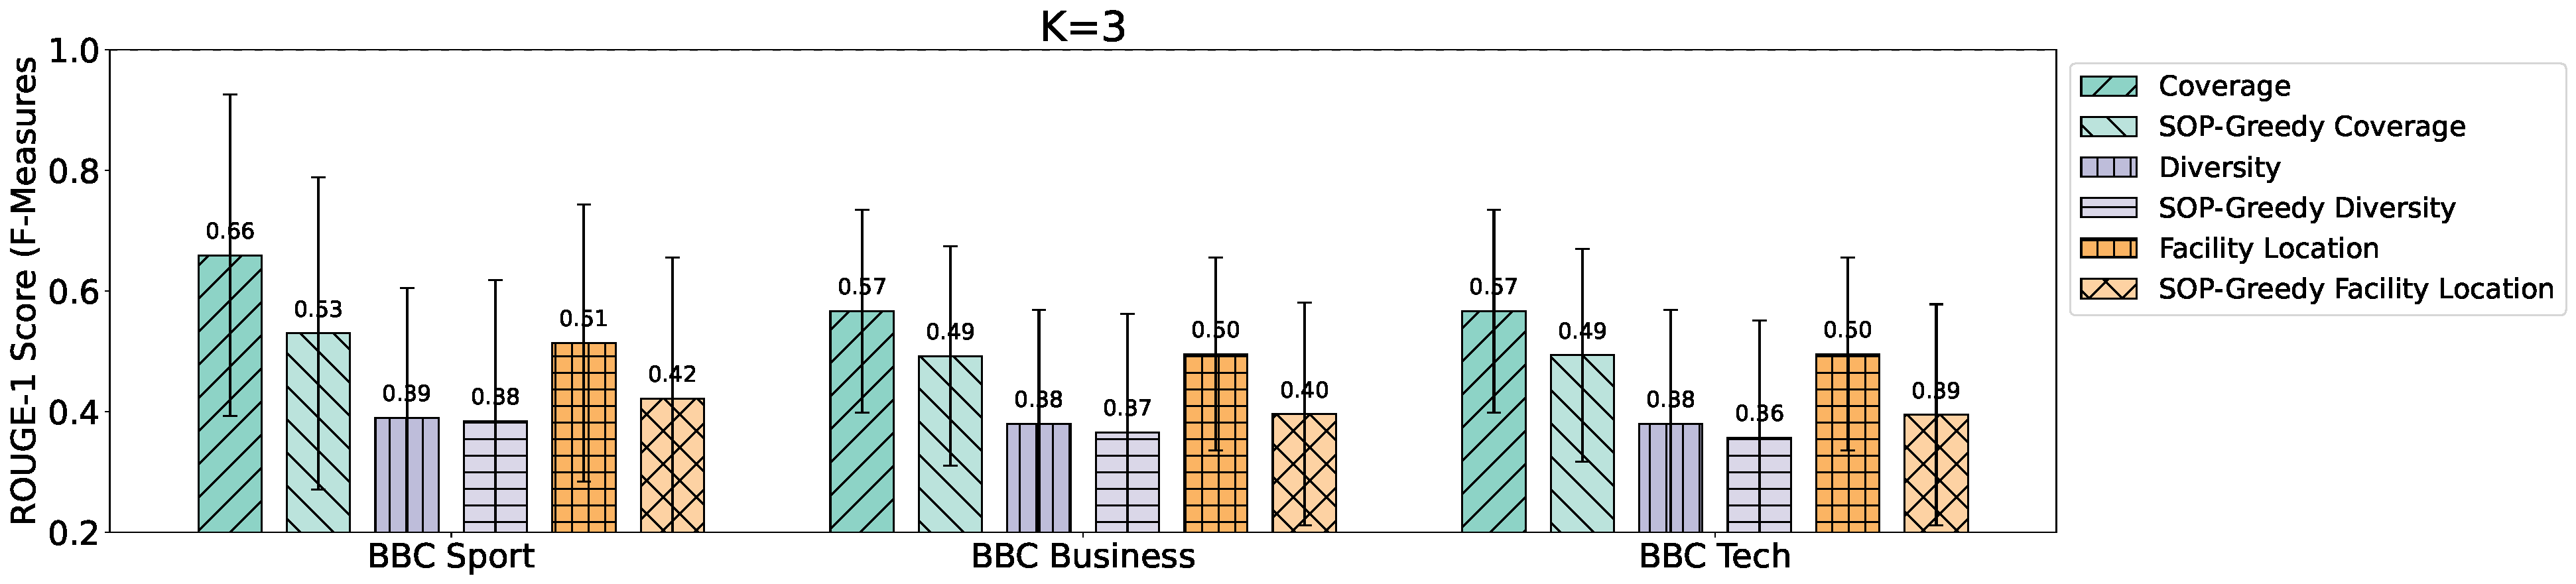
\includegraphics[width=\textwidth]{Figures/experiment 3/bbc_k3.pdf}
    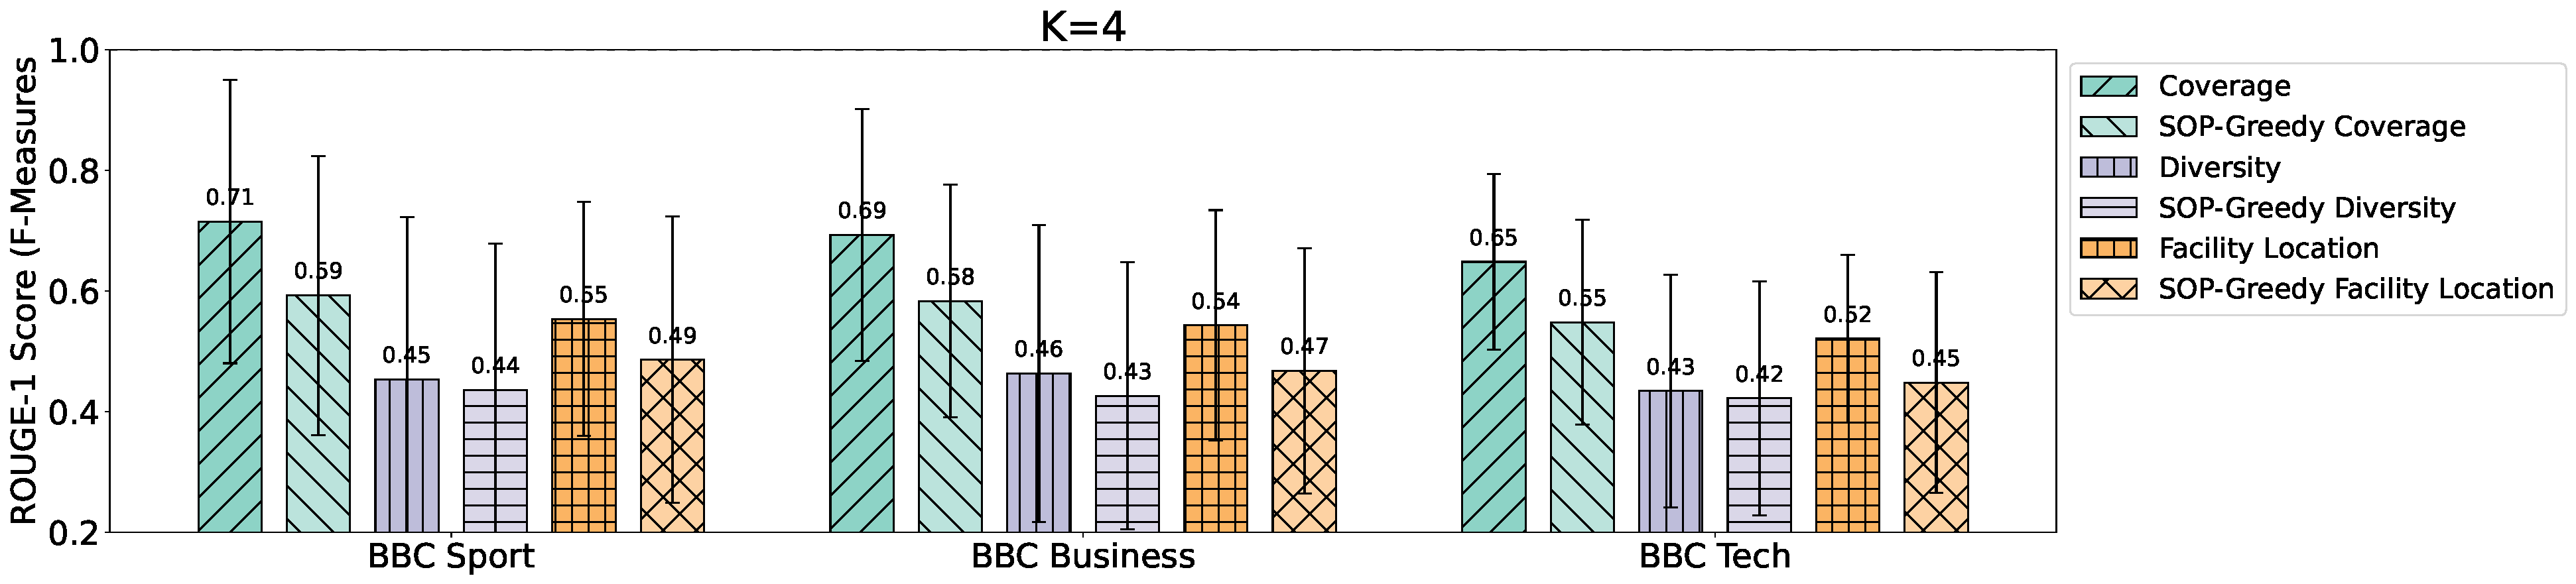
\includegraphics[width=\textwidth]{Figures/experiment 3/bbc_k4.pdf}
    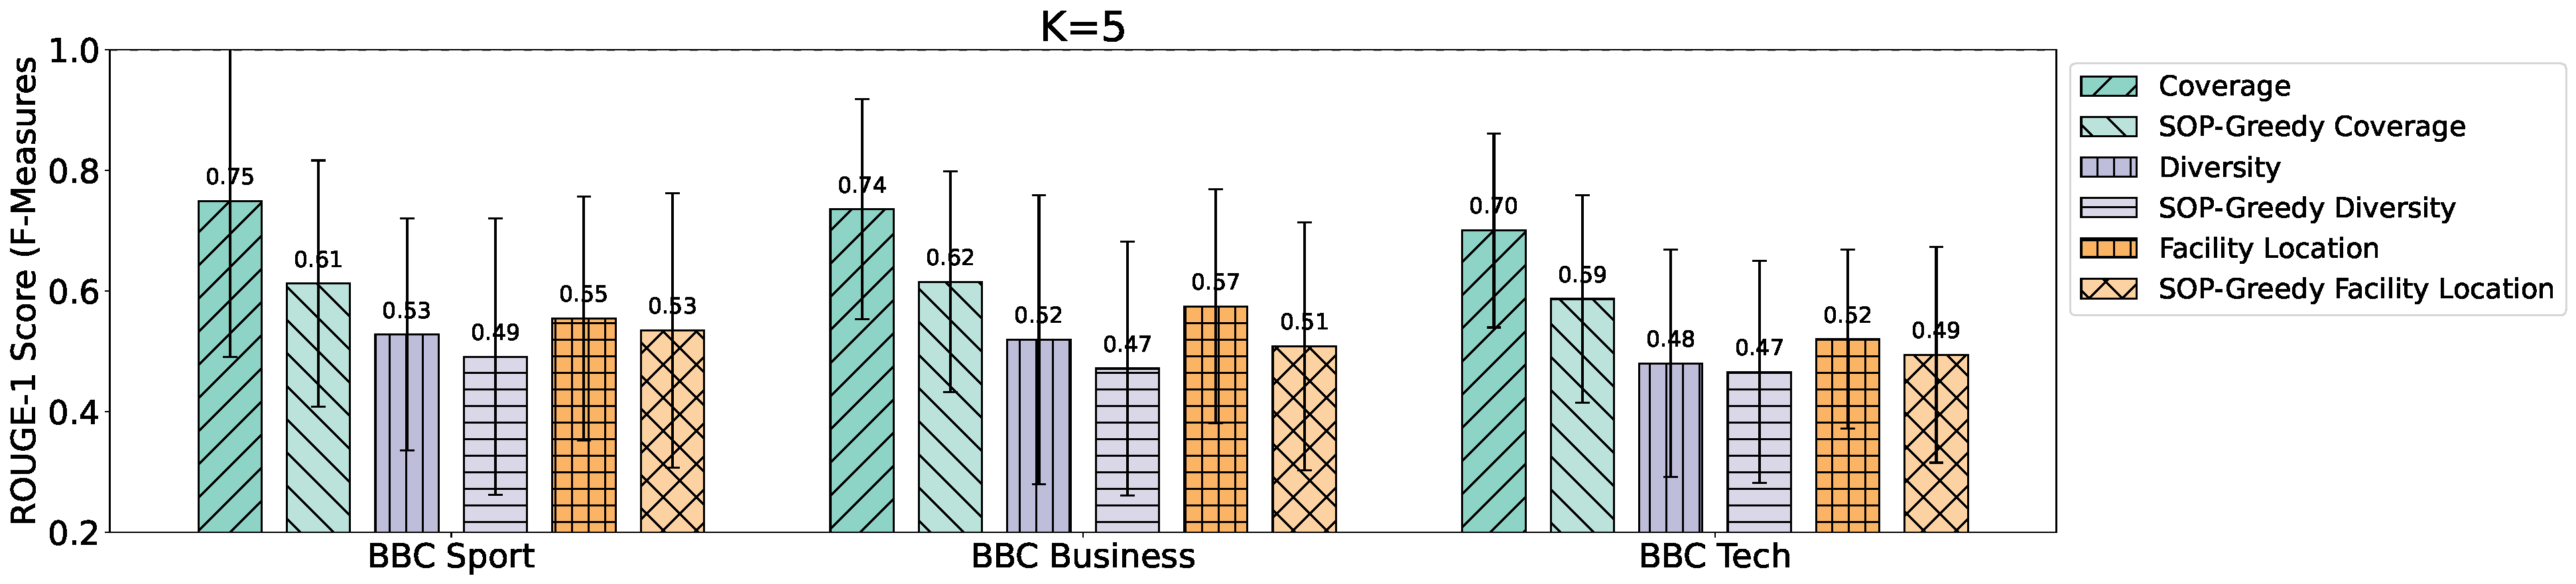
\includegraphics[width=\textwidth]{Figures/experiment 3/bbc_k5.pdf} 
    \captionsetup{aboveskip=10pt}
    \caption{Comparison of ROUGE-1 score F-measures for text summarization methods across BBC news categories and varying sentence numbers. The plot shows the performance of Coverage, SOP-Greedy Coverage, Diversity, SOP-Greedy Diversity, Facility Location, and SOP-Greedy Facility Location across BBC Sport, BBC Business, and BBC Tech datasets. Each group represents a different value of $K$, highlighting how the quantity of sentences impacts summarization quality. Error bars(IQR) indicate the variability in scores.}
    \label{fig:overall}
\end{figure}


It is observed in previous Figure \ref{fig:text-summary} that, when $K$ increases, the Rouge-1 score also improves because adding sentences in the simulated summary bring audience with valid information. When $K$ reaches a certain point, $K = 5$, the incremental information gain is insignificant. So, we make the subsequent plots across three news categories for $K = 3, 4$. Figure \ref{fig:overall} indicates that converge and facility location greedy outperform the other methods. The predictive greedy has close performance with each objective method under large prediction error value ($\eta = 100$). These findings support that submodular functions, even with prediction errors, offer a robust structure for producing short but informative summaries. Consistent performance across different $K$ values further demonstrates that the robustness of the predictive greedy generalizes to larger cardinality constraints. 

\end